\begin{samplecase}
{\bf Different alpha-particle optical model potentials: alpha + ${}^{165}$Ho}\newline
To demonstrate the variety of (spherical) optical model potentials for 
alpha-particles available in TALYS, we include a sample case in which 4 OMPs 
for alpha-particles on ${}^{165}$Ho are compared. The results are given in Fig. \ref{an} 
for the ($\alpha$,n) reaction cross sections within the incident-energy range 
of most recent measured data \cite{Glorius2014} below the Coulomb barrier.

\subsubsection{Case a: Watanabe folding approach with Koning-Delaroche nucleon potentials}
The input file is

\VerbatimInput{\samples a-Ho165-omp1/org/talys.inp}

where the file energies consists of energies between 7 and 15.5 MeV with 
0.5 MeV energy steps, corresponding to the energy range of the measured data.
This is the default calculation. Fig. \ref{an} displays the resulting 
($\alpha$,n) reaction cross sections for the target nucleus 165Ho, 
as obtained in the file rp069168.tot.

\subsubsection{Case b: McFadden-Satchler [21] potential}

The input file, using the alphaomp keyword value of 2, is

\VerbatimInput{\samples a-Ho165-omp2/org/talys.inp}

\subsubsection{Case c: Demetriou, Grama and Goriely \cite{Demetriou2002} double folding dispersive potential}

The input file, using the alphaomp keyword value of 5, is

\VerbatimInput{\samples a-Ho165-omp5/org/talys.inp}

\subsubsection{Case d: Avrigeanu et al. \cite{Avrigeanu2014} potential}

The input file, using the alphaomp keyword additional value of 6, is

\VerbatimInput{\samples a-Ho165-omp6/org/talys.inp}

where the file energies consists in addition of energies up to 33 MeV corresponding to all energy ranges which are considered in Table II of Ref. \cite{Avrigeanu2014}.
\end{samplecase}
\begin{figure}
\centering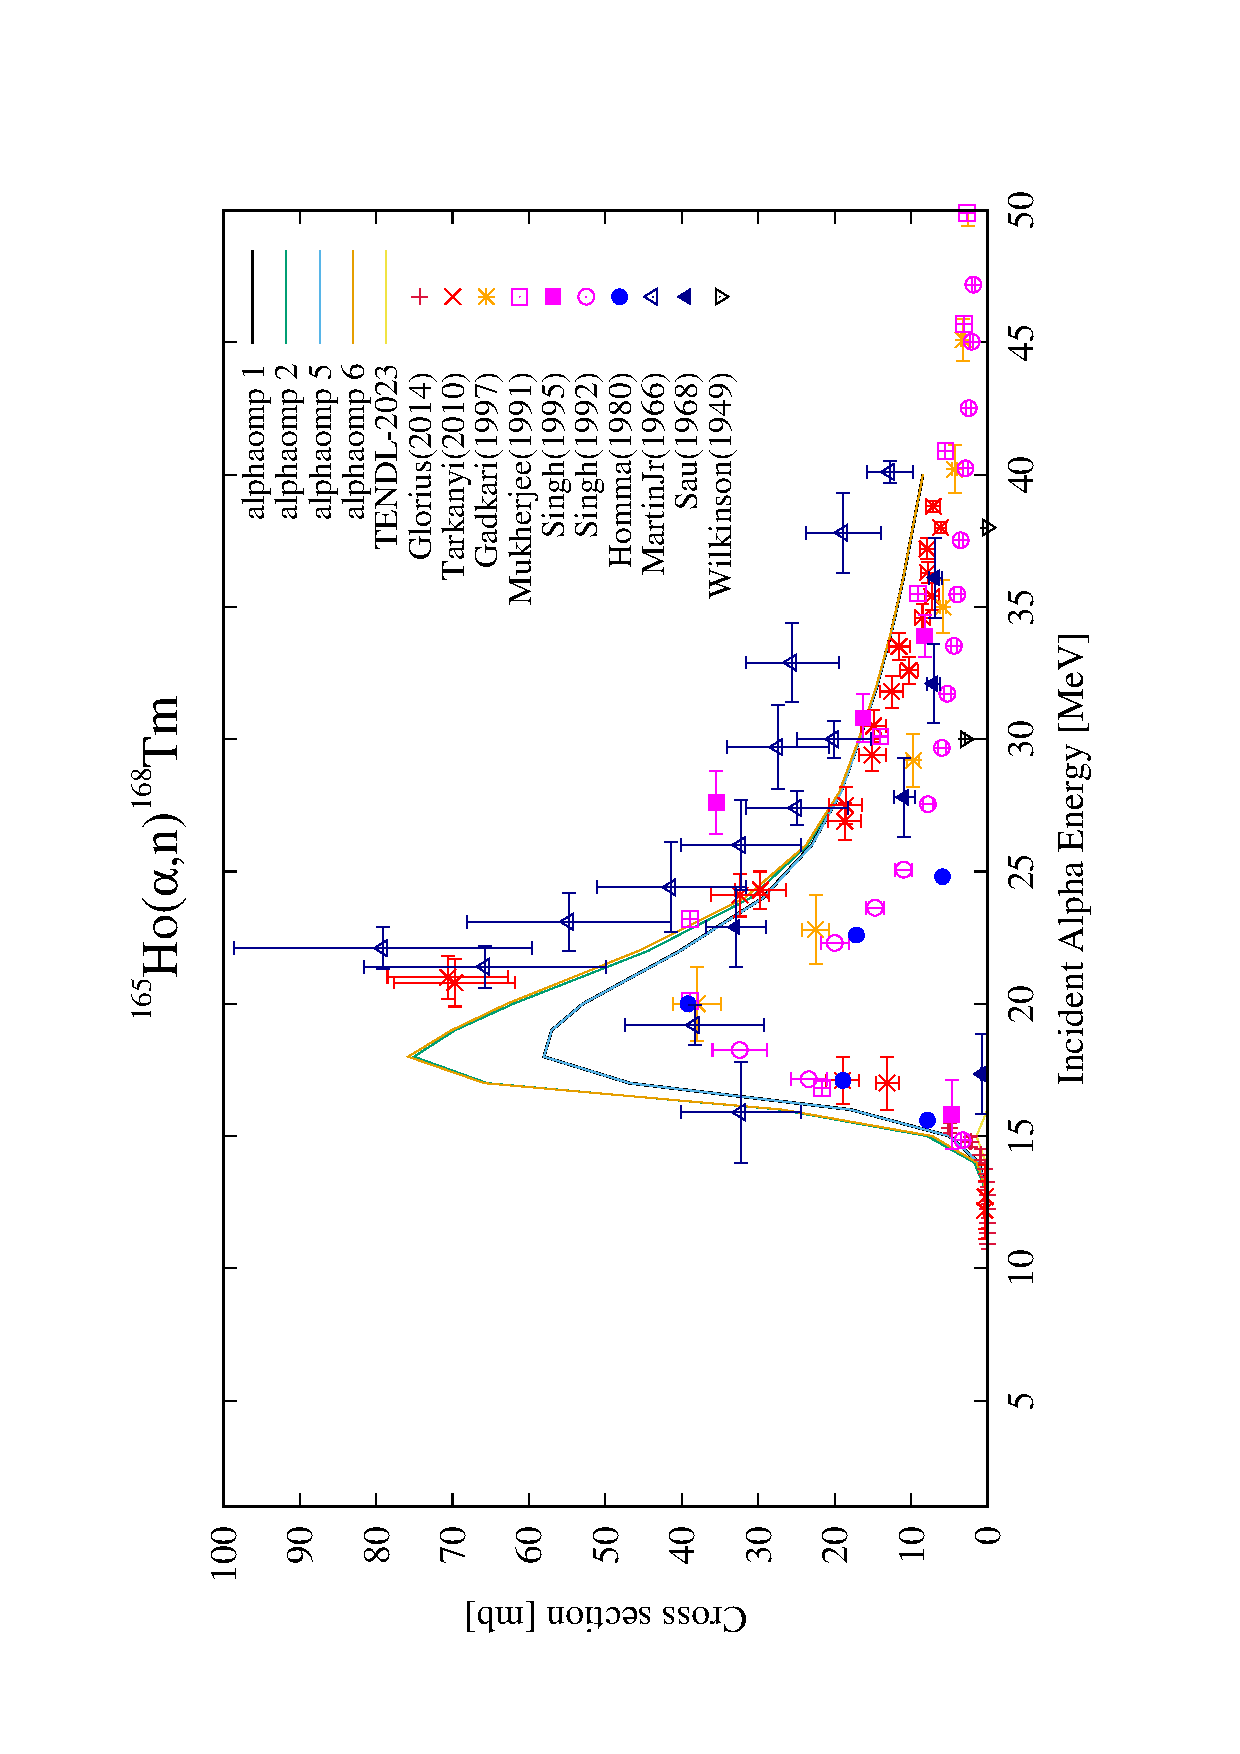
\includegraphics[scale=0.5,angle=270]{a-Ho165-omp}
\caption{$^{165}$Ho($\alpha$,n)$^{168}$Tm reaction cross sections for different OMP's.}
\label{an}
\end{figure}
